\scanpage{25}
\begin{flushright}\fbox{Algèbres de Hodge d'ordre 2}\end{flushright}
\diagram{\begin{array}{ccccc}
H^0&H^1&H^2&H^3&H^4\\
k&V&k\xi+W&\check V&k\xi^2
\end{array}}

$V,W$

\[
\bigwedge^2 V\xrightarrow{\alpha}k\xi+W
\qquad \alpha(x\wedge y)=\varphi(x,y)\xi+\psi(x,y)
\]
\[
\operatorname{Sym}^2(W)\xrightarrow{\beta}k\xi^2
\qquad \beta(xy)=Q(x,y)\xi^2
\]
\margin{$\varphi(x,y)$ forme alternée\par
$\psi(x,y)$ -- \unsure{appl.} bil. alt. dans $W$\par
$Q$ forme bil. sym. sur $W$}

\deleted{\unsure{Point de vue}}
La connaissance de $V,W,\varphi,\psi,\unsure{Q|\bar Q}$ permet de reconstituer $H^*$ :
\unsure{isom.} canonique près.

\[
H^0\times H^i\longrightarrow H^i:\quad\text{clair par}\quad
1.x=x.1=x\qquad\forall x.
\]
\[
H^1\times H^i\longrightarrow H^{i+1}\quad
\left|\begin{array}{ll}
\deleted{\unsure{donc}}\ i=1&xy=\varphi(x,y)\xi+\psi(x,y)\qquad x,y\in V\\
i=2&\begin{array}{l}
x\xi=\xi x=\widetilde\varphi(x):\quad\deleted{\unsure{(*)}}\ y\longmapsto\varphi(y,x)\\
xw=wx=\unsure{\rho'|\rho^1}(w,x):\quad y\longmapsto Q(\psi(y,x),w)
\end{array}\quad\left|\begin{array}{l}x\in V\\y\in V\\w\in W\end{array}\right.\\
i=3&xy'=-y'x=\unsure{\langle x,y'\rangle|+\langle x,y'\rangle}\xi^2\qquad x\in V,y'\in\check V\\
\deleted{\unsure{i=4}}&\deleted{\unsure{x\xi^2=0}}
\end{array}\right.
\]
\[
H^2\times H^i\longrightarrow H^{i+2}\quad
\left|\quad i=2:\quad\left|\begin{array}{l}
\xi.\xi=\xi^2\\
\xi w=w\xi=0\quad(w\in W)\\
ww'=Q(w,w')\xi^2
\end{array}\right.\right.
\]
\figure{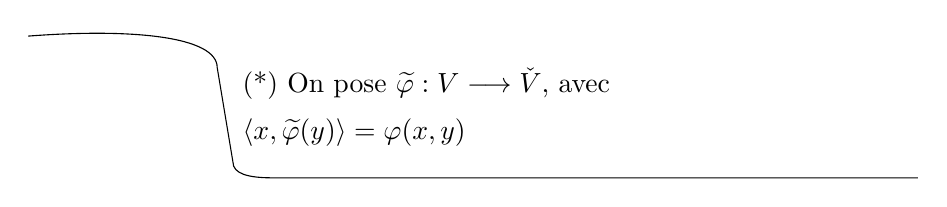
\begin{tikzpicture}[x=1cm,y=1cm]
\node[anchor=west,align=left] at (.2,0) {(*) On pose $\widetilde\varphi:V\longrightarrow\check V$, avec\\[.5em]$\langle x,\widetilde\varphi(y)\rangle=\varphi(x,y)$};
\draw (-2.4,.9) .. controls (-1.1,1) and (0,.9) .. (0,.5) -- (.2,-.7) .. controls (.2,-.85) and (.4,-.9) .. (.7,-.9) -- (8.9,-.9);
\end{tikzpicture}}

\unsure{Quelle que soit la donnée} de $\varphi,\psi$, on trouve une loi de composition
anticommutative, admettant $1$ comme unité.

\uline{Condition d'associativité} s'écrit $(xy)(tz)=(tx)(yz)$, sous la forme
\[
\deleted{\unsure{(*)}}\quad
\boxed{\varphi(x,y)\varphi(t,z)+Q(\psi(x,y),\psi(t,z))
=\varphi(t,x)\varphi(y,z)+Q(\psi(t,x),\psi(y,z))}
\]
\margin{Exprime aussi que la forme $(xy)(zt)$ en $xyzt$ est alternée en $y,z$
(donc en \unsure{toutes les var.!|tous les var.!})}

\uline{Condition de Lefschetz}
\[
\xi^2:H^0\simeq H^4\qquad\text{tjrs satisfait}
\]
\[
\xi:H^1\longrightarrow H^3\qquad\text{ssi}\quad
\boxed{\varphi\text{ non dégénérée}}
\]

\uline{Condition de Poincaré}
\[
\begin{array}{l}
H^4\simeq k\quad\text{tjrs satisfait}\\
H^0\times H^4\longrightarrow H^4\text{ et }H^1\times H^3\longrightarrow H^4\quad\text{non dég.: }\uline{\text{it\unsure{ou}}}\\
H^2\times H^2\longrightarrow H^4\quad\text{non dég ssi}\quad\boxed{Q\text{ non dégénérée}}
\end{array}
\]
\mspage{24}
